\section{Data}
\label{sec:data}

In the following chapter, the collection, processing and validation of the relevant data will be explained. The empirical data is collected from public projects on GitHub until February 2016 \footnote{collected during the period from December 2015 to February 2016}. Repositories' related activity data is analyzed from 2011 to 2015.

Beside the selection of languages (see chapter \ref{sec:selection_of_programming_languages}) and firms (see chapter \ref{sec:firms_are_relevant_commercial_organizations}) all analyzed observations are unfiltered \footnote{unless stated otherwise} and contain the full available range of public available firms' OS projects.

\textit{Git} is an OS distributed version control system. It is published and developed by the \textit{Linux} development community (including Linus Torvalds, the creator of \textit{Linux}) since 2005 \cite[p.31]{chacon2014pro}.

\subsection{Data Sources and Open Data Approach}

All analyzed data is collected from the following public and free available data sources:

\begin{itemize}
	\item [\textbf{GitHub API:}] Project data, issues and issue comments
	\item [\textbf{Git repository:}] Code contribution
	\item [\textbf{Glassdoor API:}] \footnote{\url{https://www.glassdoor.com/developer/index.htm}} Firm and employee's ratings
	\item [\textbf{GitHub Archive:}] \footnote{\url{https://www.githubarchive.org/}} Time-referenced data for user events (time period 2011 - 2015)
	\item [\textbf{GHTorrent Project:}] \footnote{\url{http://ghtorrent.org/}} User data (email, location, company and full-name)
	\item [\textbf{LinkedIn Websearch:}] Manual classification for developer employments
\end{itemize}

External data is received as JSON files (\cite{bray2014javascript}) and converted to the CSV format (\cite{shafranovich2005common}) for better processing possibilities in \textit{R}. All data can be downloaded and observed through a git repository \footnote{\url{https://git.zeitpulse.com/philipp/masterthesis-data/tree/master}}.

\clearpage
\subsection{Selection of Programming Languages}
\label{sec:selection_of_programming_languages}

To specify a proper selection of relevant OS projects we need to define a list of popular programming languages.

The most used programming languages on \textit{GitHub} \footnote{\textit{Visited 12.01.2016:  \url{https://github.com/search?o=desc&q=stars:\%3C1}}} are listed in table \ref{tbl:github_language_distr_top_repos} (\cite{GitHubTrendingLanguages2015}). The figures reflect the overall ranking of programming languages in OS (\cite{GithubsTopCodingLanguagesShowOpenSourceHasWon:online}) and integrates close enough to the \textit{TIOBE index} (\cite{TIOBE2015}) and \textit{Programming languages used in most popular websites} on \cite{ProgrLangPopWeb2015}. Excluded languages are \textit{Shell} and \textit{CSS} since \textit{Shell} is a UNIX command line interpreter and neither used for building regular web services nor for building software in the proper sense \footnote{ \url{http://www.rpi.edu/dept/arc/training/shell/slides.pdf}} and \textit{CSS} is a markup language and not a programming language.

The replacement of \textit{Shell} and \textit{CSS} with the \textit{GO language} seems to be reasonable (see \cite{JavaReignsButGoLanguageSpikesInPopularity:online}, \cite{ThePopularityOfGo:online} and \cite{WhyGooglesProgrammingLanguageCanRivalJava:online} for possible reasons). The selection excludes the "rising stars" of OS programing languages \textit{Scala, Hack} and \textit{Swift} since the popularity, spreading and age of those languages is too little for the observation.

The following 10 languages (in alphabetically order, grouped by programming language family) are finally selected:

\begin{itemize}
	\item C, C\#, C++, Objective-C
	\item Go
	\item Java
	\item JavaScript
	\item PHP
	\item Python
	\item Ruby
\end{itemize}

The exact number of projects according to \textit{Stars} and \textit{Forks} can be looked up in table \ref{tbl:github_language_distr_top_repos} and figure \ref{fig:github_popular_programming_languages} respectively.

The usage of programming languages in projects differ between firms. Some firms promote their own programming languages (e.g. \textit{Google} uses \textit{Go} / \textit{Microsoft} uses \textit{C\#} more often than usual) or use specific languages according to their field of application (e.g. \textit{GitHub Inc.} uses \textit{Ruby}). Figure \ref{fig:programming_language_use_by_firms} and
\ref{fig:languages_used_in_projects} illustrate the usage of the 10 selected programming languages in "Top Projects" and "Residual Projects" \footnote{terms will explained on page \pageref{sec:top_and_residual_projects}} according to firms.

\begin{figure}[!h]
	\centering
	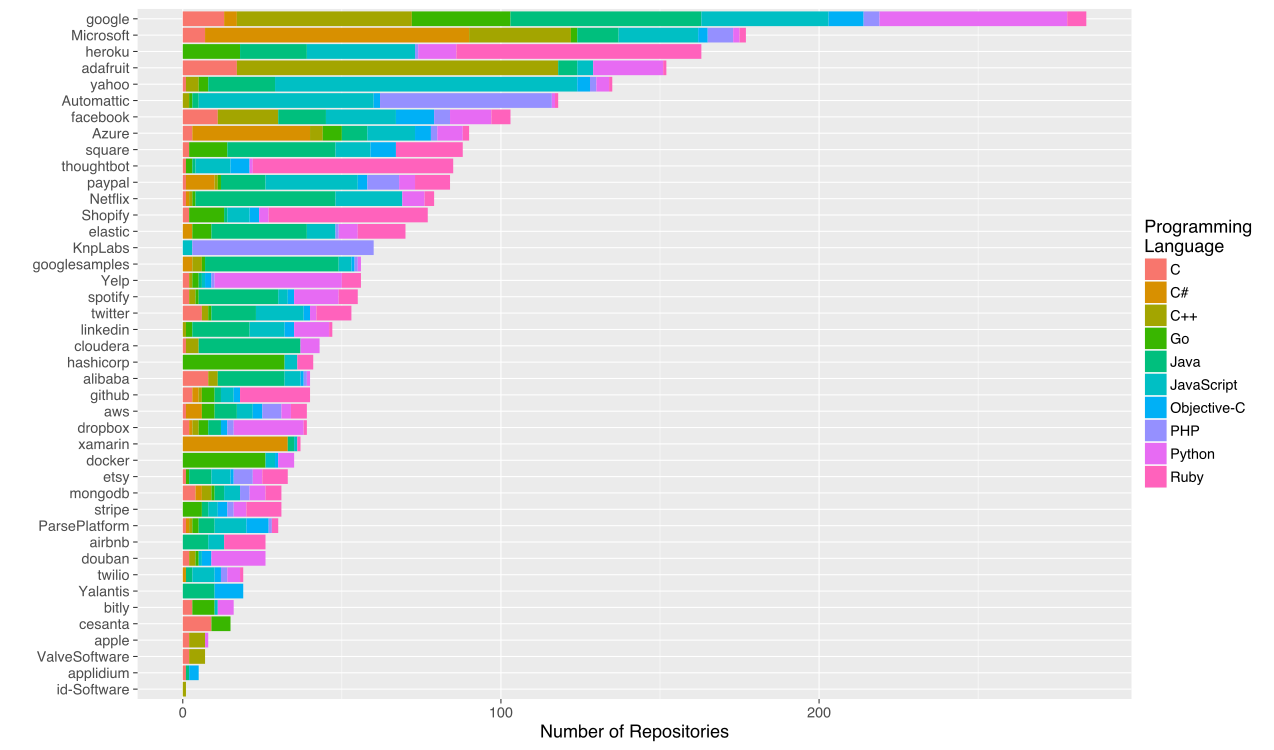
\includegraphics[page=1,scale=0.45]{../graphics/intro/programming_language_use_by_firms.pdf}
	\caption{OS Projects of Firms and the Programming Languages they are written in}
	\label{fig:programming_language_use_by_firms}
\end{figure}

\begin{figure}[!h]
	\centering
	\includegraphics[page=1,scale=0.45]{../graphics/intro/languages_used_in_projects.pdf}
	\caption{Programming Languages which are used in \textit{Top Projects} and \textit{Residual Projects}.}
	\label{fig:languages_used_in_projects}
\end{figure}

\begin{table}[!h]
\centering
\begin{tabular}{lll}

\hline
\textbf{Programming language} & \textbf{Stars} & \textbf{Forks} \\ \hline
JavaScript        & 252891        & 134294         \\
Python            & 132995        & 74924          \\
Java              & 115249        & 83361          \\
Ruby              & 105547        & 55153          \\
PHP               & 97112         & 57332          \\
C                 & 59920         & 36506          \\
C++               & 53706         & 33105          \\
Objective-C       & 44734         & 24845          \\
C\#               & 35859         & 22157          \\
Shell             & 36874         & -              \\
CSS               & -             & 21637          \\ \hline
\textbf{Sum}      & \textbf{934887}     & \textbf{733789}         \\ \hline

\end{tabular}
\caption{Programming Languages with projects' \textit{Stars} and \textit{Forks} (\textit{Retrieved: 12.10.2016})}
\label{tbl:github_language_distr_top_repos}
\end{table}


\clearpage

\subsection{Restrictions of Data Collections}

All measurements and analyses are made under the following restriction: GitHub repositories' social data (\textit{stargazers}, \textit{forks}, \textit{contributors}, …) can only be measured with the actual values, i.e. cross-sectional data. For that reason, these attributes are query able through the GitHub API (\cite{GitHubApi}) with the possibility of sorting. However, querying and analyzing time series of GitHub event data is possible through the GitHubArchive (see \cite{grigorik2012github}; \cite{AnalyzingMillionsOfGitHubCommits:online}; listing \ref{lst:githubusersandprojectscount}) having events with the verbs \textit{watch} (mostly called \textit{subscribing}) and \textit{fork}. As mentioned in the beginning, the available time period of user activities is from 2011 to 2015 \footnote{GitHub itself exists since 2007 (\cite{GitHubCEOAndCo-FounderChrisWanstrathKeynoting:online})}.

\subsection{Social-Success-Metrics of git Repositories}
\label{sec:social-success-metrics}

A \textit{git repository} (sometimes also called \textit{git project} or \textit{git repo}, where \textit{git} is an optional term) provides the following statistics by default:

\begin{itemize}
	\item date and time of commits (commits are code contributions)
	\item name and email of the author (authors are developers)
	\item time zone location of the contributor (via the date-time property)
	\item code changes and action \footnote{an action may be a regular \textit{code commit}, \textit{code merge} or basic file operation (like rename, delete, copy or create file)}
\end{itemize}

A GitHub project has the following social metrics (terms will be described in the paragraph below):

\begin{itemize}
	\item Stars / Stargazers
	\item Subscribers (sometimes also called "Watchers")
	\item Forks
	\item Open and closed Issues
\end{itemize}

Finally, we get the following metrics of interest:

\begin{itemize}
	\item Number of Stargazers, Subscribers and Forks
	\item Number of Code Commits
	\item Number of Contributors
	\item Number of Issues and Comments on Issues
\end{itemize}

\textbf{Stargazers} \footnote{derived "action" is \textit{Star}} are GitHub users / developers who mark a project with a star (\cite{GitHubStargazers}), similar to the ordinary "like button" on \textit{facebook}. The reason may be to mark this as one of your favorite projects or to show the initiator your interest in the project or idea.

\textbf{Fork} is a copy / clone of a git project (\cite{GitHubForks}) containing all previous code contributions until the moment of the fork event. Projects are forked either to collaborate with the origin project or to be resumed as an independent project \footnote{\textit{LibreOffice} is a fork of \textit{OpenOffice} which is continuing as independent project for instance}. The number of forks doesn't explain necessarily the activity of contributors nor the popularity. If you participate on a GitHub project by committing code (called \textit{pull request} \footnote{\url{https://help.github.com/articles/using-pull-requests/}}) with your GitHub account, this project will be forked into your account by default. The \textit{clone} and \textit{fork} actions are fundamental ideas of the decentralized approach of git (\cite{loeliger2006collaborating}).

\textbf{Subscribers} are users who get notified on important project activities (\cite{GitHubWatchers}). The term is similar to \textit{subscribing} on \textit{facebook} or \textit{following} on \textit{twitter}. \textit{Subscribing} may be considered as the most important indicator of active interest in projects (beside code contribution and issue participation).

\textbf{Issues} are communication threads (\cite{GitHubIssues}). Every issue can be \textit{open} or \text{closed} and labeled as \textit{feature request}, \textit{bug report}, \textit{idea} or \textit{code proposal} for instance. Issue threads are an exclusive collaboration feature of GitHub \footnote{\url{https://guides.github.com/features/issues/}} and not implemented in git itself.

In terms of \textbf{"Forms of Participation"} (see chapter \ref{sec:forms_of_participation_on_github} and figure \ref{fig:forms_of_commitment} respectively) we can roughly classify this (direct and indirect) user actions from "lower participation / activity" to "higher participation / acitivity". \textit{Stars} and \textit{Forks} can be interpreted as the lowest participation level because they do not influence projects' progress directly (everyone can \textit{fork} and \textit{star} a project without any direct "consequences"). Whereas \textit{subscribing} is more active (but still indirect), because it provides constant updates of the current project activities to the subscribing user.

The impact of internal (and external) contribution on these levels of participation has to be considered specifically. In general, higher-active responses are more important than lower-passive responses.

\clearpage
\subsection{Projects' Data Enquiry}

Due to GitHub API limitations (\cite{GitHubApiLimit}) we are only able to query 1000 results for each language. As mentioned before, only firm's initiated projects for the 10 most famous programming languages are interesting for the observation.

By querying the most popular 1000 repositories for each of the programming languages \footnote{for each language:  \url{https://api.github.com/search/repositories?q=language:$ProgrammingLanguage$&sort=stars&order=desc&per_page=100&page=1...10}, queried on 19.1.2016} we finally receive 10,000 repositories \footnote{\url{https://git.zeitpulse.com/philipp/masterthesis-data/tree/master/apidata/top_repos_by_language}} from 2858 different organizations \footnote{\url{https://git.zeitpulse.com/philipp/masterthesis-data/raw/master/csv/organizations.csv}}, sorted descending by listed "Top Repositories" for each organization \footnote{in the following top repositories or top projects are all projects listed in the top 1,000 search matches} (see table \ref{tbl:organizations_with_top_repos} on page \pageref{tbl:organizations_with_top_repos}).

This results in 2,858 organizations having 78,055 public repositories (see table \ref{tbl:rep_numbers_organization} for details  \footnote{\url{https://git.zeitpulse.com/philipp/masterthesis-data/raw/master/apidata/organizations_top_repos_restructured.json}}). By selecting the most relevant organizations \footnote{i.e. having at least 4 different projects in the search results of most popular projects on all 10 programming languages} we get 113 (share of 3.95 \%) relevant organizations \footnote{data source: \url{https://git.zeitpulse.com/philipp/masterthesis-data/raw/master/csv/repositories_details.csv}}. We can classify finally 58 relevant commercial firms (see table \ref{tbl:selected_commercial_firms} and chapter \ref{sec:firms_are_relevant_commercial_organizations}).

Evidently, closer examination of the data shows that nearly every commercial successful firm in the technology area has a public GitHub profile (see table \ref{tbl:commercial_successfull_firms_on_github_with_languages} on page \pageref{tbl:commercial_successfull_firms_on_github_with_languages}).
%
% \subsubsection{Top and residual Repositories}

\label{sec:top_and_residual_projects}

We classify \textbf{Repositories} as:

\begin{itemize}
	\item[\textbf{Top Repositories}] (sometimes also called \textit{Top Projects}), which were found the first 1,000 rank search result
	\item[\textbf{Residual Repositories}] are the remaining amount of repositories by each firm
\end{itemize}

All firms' projects that are classified in one of the 10 chosen programming languages and are not tagged as "fork" are relevant \footnote{Remark: Unfortunately, not all projects can be classified absolutely as \textit{fork} and \textit{not fork} since not all projects are tagged as such on GitHub itself}.

\begin{table}[!h]
\centering
\begin{tabular}{ll}
Popular / Top Repositories:  						& 10,000         	\\
Repositories by Organizations:		& 78,055					\\
Organizations:  									& 2,858          \\
Organizations with relevant Number of Top Repositories:  					& 113          \\
Commercial Organizations:  					& 58          \\
Share of relevant Organizations:  & \textbf{3.954 \%}		\\
Share of observed Organizations:  & \textbf{2.03 \%} \/ \scriptsize{(51.33 \%)}
\end{tabular}
%\hspace{\textwidth}
\caption{Top Repositories for selected Programming Languages on \textit{GitHub}. "Share of observed Organizations" are finally classified commercial firms (selection criterions will be explained in chapter \ref{sec:firms_are_relevant_commercial_organizations})}
\label{tbl:rep_numbers_organization}
\end{table}

\clearpage
\subsection{Firms are relevant commercial Organizations}
\label{sec:firms_are_relevant_commercial_organizations}
A firm is relevant for the study, if

\begin{itemize}
	\item it is a commercial organization
	\item uses at least one of its projects actively in their business
	\item it contributes source code to their own projects and to other OS projects
	\item it holds and uses a global web domain \footnote{an actively used web domain is important to classify firm employed and external developers}
\end{itemize}

The selection was done manually by evaluating the form of company, activity with employed developers and firms' business activity. Since the classification of commercial activity is qualitative, it is also based on ratings by employees on Glassdoor \footnote{\url{https://www.glassdoor.com/}} \footnote{\url{https://git.zeitpulse.com/philipp/masterthesis-data/tree/master/apidata/glassdoor/employers}}, which will be introduced in chapter \ref{sec:glassdoor_ratings}.

We will evaluate the repositories of these firms \footnote{\url{https://git.zeitpulse.com/philipp/masterthesis-data/blob/master/csv/repositories.csv}} and compare participation of firm employed and external developers.

The assessment of which organization is commercial and builds a business on its OS projects follows the assumption that:

\begin{itemize}%[a)]
	\item most projects are used by the firm in commercial context (like \textit{docker, aws} ...)
	\item the firm offers paid services for some of its project (like \textit{chef, Microsoft, } ...)
	\item the firm acts commercial - even the OS projects and their service is available for zero costs (like \textit{GitHub, facebook} ...)
\end{itemize}

\subsection{Structure of a git Project}

A git repository can roughly be described with the following attributes \cite[p.~32]{loeliger2012version}:

\begin{itemize}
	\item commits, tags and merges
	\item branches
	\item trees \textit{(not relevant here)}
	\item files / blobs \textit{(not relevant here)}
\end{itemize}

A detailed explanation of those attributes is not necessary because only \textit{commits} and \textit{branches} are relevant for the study and will be explained in the following chapters.

\subsection{Branches of Interest}

Each git repository contains different branches. Every branch can be a different working subtree (i.e. source code environment) of a project. We will only inspect the default branch of each project which is in most cases the \textbf{master branch}. The master branch is by convention the official branch containing all finally submitted and accepted code of a project \cite[p.~89-90]{loeliger2012version}. Some projects have different default branches (\textit{production} branch for instance) and will be scope of the observation if it is tagged as such on GitHub.

% \subsection{Used Programming Languages by Firms}

\subsection{Firms' License Usage}
\label{sec:firms_and_licenses}

Which kind of licenses firms are using might reflect their strategic and projects' commercial long-term intention respectively.

With the following segmentation (based on \cite{bonaccorsi2003licensing}) for the most used licenses of the observed repositories / firms, we can describe a spectrum from restrictive to permissive licenses. As figure \ref{fig:licenses_used_by_firms} illustrates: most firms use (very) permissive licenses (from green-blue to magenta) instead of restrictive licenses (red to orange) \footnote{which is in line with \cite{bonaccorsi2003licensing} and \cite{top20oslicenses:online}}. The reason might be simple: Permissive license avoid problems of the copy-left idea and enables future commercial (closed source) development.

\begin{figure}[!h]
	\centering
	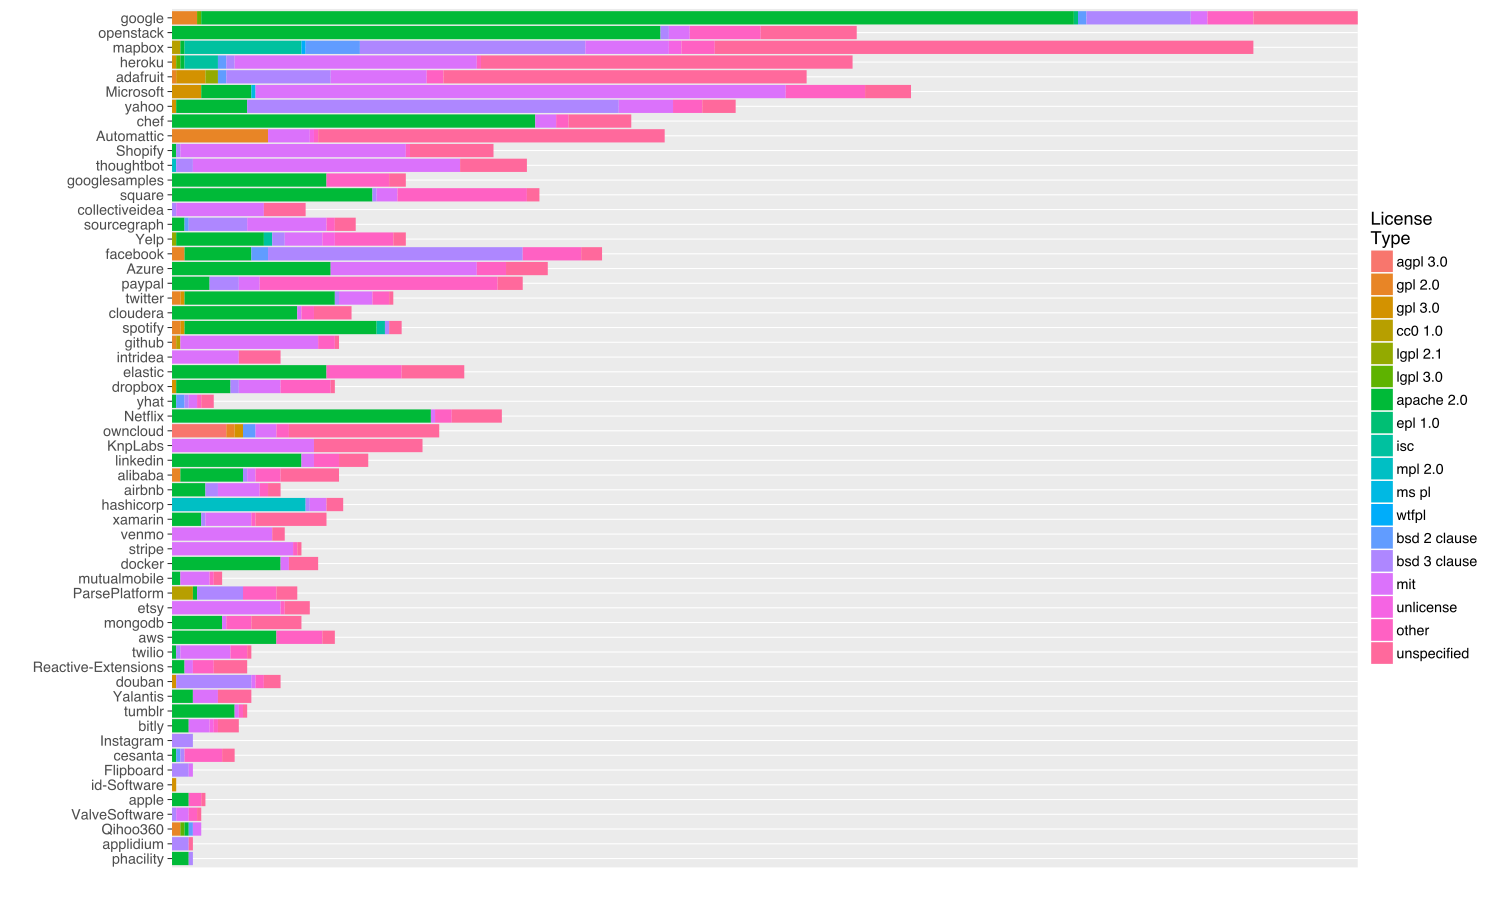
\includegraphics[page=1,scale=0.3]{../graphics/intro/which_firm_is_using_which_license.pdf}
	\caption{Most OS projects by firms do use (very) permissive licenses (from green over blue to magenta). The x-axis (caption not in the plot) represents the absolute number of repositories (from 15 - 284 repositories).}
	\label{fig:licenses_used_by_firms}
\end{figure}

\begin{figure}[!h]
	\centering
	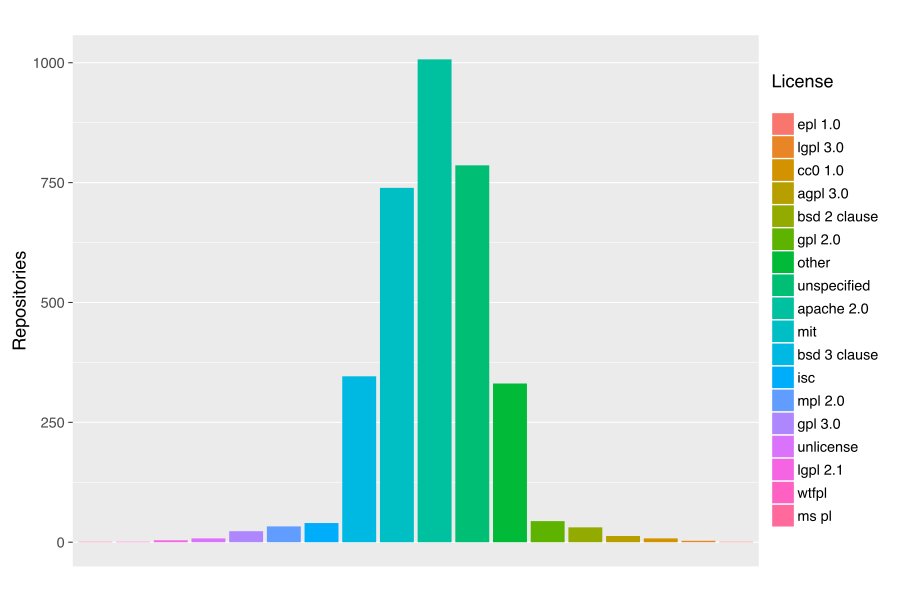
\includegraphics[page=1,scale=0.4]{../graphics/intro/licenses/popular_licenses.pdf}
	\caption{Frequency of licenses in GitHub repositories of firms. Permissive licenses (like Apache, MIT and BSD) are favored. \textit{Unspecified} means not categorized (i.e. in most cases proprietary OS license by firm). Graphs for Top and Residual Projects in figure \ref{fig:licenses_in_residual_projects} and \ref{fig:licenses_in_top_projects}.}
	\label{fig:licenses_in_projects}
\end{figure}

\clearpage
\textbf{Strong Copyleft (restrictive)}

\begin{itemize}
	\item GNU Affero General Public License (agpl 3.0)
	\item GNU General Public License (gpl 2.0, gpl 3.0)
	\item Creative Commons CC0 1.0 Universal (cc0 1.0)
	\item SIL Open Font License (ofl 1.1)
\end{itemize}

\textbf{Mixed (less restrictive, more permissive)}

\begin{itemize}
	\item GNU Lesser General Public License, Version 2.1 (lgpl 2.1, lgpl 3.0)
	\item Apache License, Version 2.0 (apache 2.0)
	\item Eclipse Public License (epl 1.0)
	\item ISC-Licence (isc)
	\item Mozilla Public License, version 2.0 (mpl 2.0)
	\item Microsoft Public License (ms pl)
\end{itemize}


\textbf{Non-Copyleft (very permissive)}

\begin{itemize}
	\item Do What The Fuck You Want To Public License (wtfpl)
	\item BSD licenses (bsd 2 clause, bsd 3 clause)
	\item The MIT License (mit)
\end{itemize}

\textbf{Uncategorized}

Beside that there are also unlicensed projects (i.e. no license on "purpose") and license unspecified projects (i.e. no license detected by GitHub).

\subsection{Classification of Developers}

We distinguish two groups of participants:

\begin{enumerate}
	\item [\textbf{1) Internal Developers}] (also called \textit{firm employed developers}) are developers / users who
	\begin{itemize}
		\item are currently employed at the company of the observed project, or
		\item were employed at the company of the observed project in the past
	\end{itemize}
	\item [\textbf{2) External Developers}] are developers / users who
	\begin{itemize}
		\item never worked at the company of the observed project, and / or
		\item are independent developers / hobbyist programmer
	\end{itemize}
\end{enumerate}

\subsection{Evaluation and Classification of Commits}

A \textit{commit} represents the participation of a developer. It includes code changes or new code \footnote{detailed code changes can be inspected by \textit{git diff \$commithash}}. In the following, we will regard a commit as a participation activity. We ignore the size of the commit (how many lines and files have changed) because measuring code quality by these simple metrics would be difficult. According to \cite{stamelos2002code} further specialized software is needed to measure code quality reliable.

The number of projects' valid commits of the selected 58 firms is 2,951,188. These commits are used in the final version of the projects (i.e. they are productive code commits). Commits without a valid email address \footnote{here a valid email address following ABNF with the regular expression
\tiny{\verbatiminput{../listings/w3c_html5_email.regex}}
Source: \url{http://www.w3.org/TR/html5/forms.html\#valid-e-mail-address}
} are sorted out. As mentioned before, a commit can also be a \textbf{merge} and is taken into account as well \footnote{\textit{Merge} is an activity of implementing proposed code changes into the (final) project}.

There are 1,111,384 of firm employed developers and 1,839,804 of external developers \footnote{for classification see next section}. Thus, the share of firm employed developers is at least 37.66 \% on all observed projects.

To compare the participation of firm employed and not firm employed developers, each commit must be identified by the author's email address and be assigned to internal (i.e. employed by firm) or external (i.e. employed not by firm of the project). The selection of firm employed developers is quite conservative, because we only regard developers with a firm e-mail address or developers which are known to work for the company. Many more developers may work or have been working for the firm in the past.

To maximize the classification of firm employed developers with acceptable effort, a whitelist was generated and checked manually via LinkedIn for the developers with the highest share of participation. The whitelist \footnote{can be received as csv file: \url{https://git.zeitpulse.com/philipp/masterthesis-data/raw/master/csv/classification/int_ext_developer_classification.csv}} contains over 550 manually checked developers, everyone with a share of code contribution from 25 \% up to  100 \% for a specific project.

\subsection{Time and Location of Code Contribution}

Through almost 3 Mio. observed commits we can measure a representative frequency of code contribution (see figures \ref{fig:distribution_developer_commits_by_timezone}, \ref{fig:distribution_developer_commits_local}, \ref{fig:distribution_developer_commits_wordlwide} and \ref{fig:distribution_developer_commits_by_month}). The histograms are stacked and not overlaid \footnote{the total number of commits by not firm employees is actually higher (see previous section for numbers)}.

\textbf{Interpretation}: Most of the code contribution takes place between 9:00 and 19:00 with its peak at 15:00 (see table \ref{fig:distribution_developer_commits_local}). An interesing observation is that firm employed developers' and external developers' code contributions frequency is very similar. The reasons could be:

\begin{enumerate}[a)]
	\item external developers are employed as well (but at another firm)
	\item externals / freelance workers write and commit code in the same time frame because they are most efficient in that time frame
	\item externals / freelance workers write and commit code in the same time frame because code contribution is a form of collaboration and "forces" same time frames
\end{enumerate}

According to the manual classification of developers (most of them are or were employed at the particular firm) and the fact that code contribution time is similar regarding to the local time, reason a) seems to be the prime cause: \textbf{external developers are employed developers of other / rival firms}.

Beside that, the core hours are in line with independent studies about working hours (see figure \ref{fig:us_standard_workday}). Thus, the most effective time period for developers seems to be between midday and late afternoon. The distribution of worldwide code contribution confirms the leading role of Silicon Valley / California / Oregon and USA in the firm managed open source segment (see figure \ref{fig:distribution_developer_commits_by_timezone} and  \ref{fig:distribution_developer_commits_wordlwide})

\begin{figure}[!ht]
	\centering
	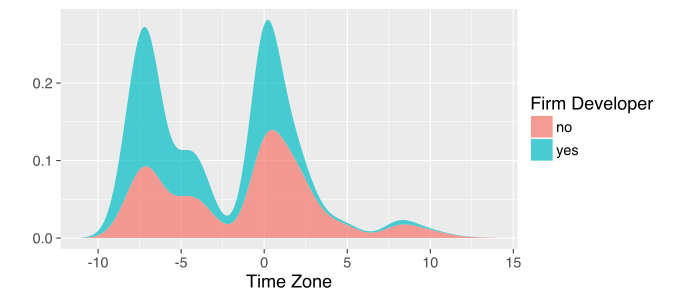
\includegraphics[page=1,scale=0.7]{../graphics/intro/timezone_of_code_contribution.pdf}
	\caption{Code contributions by firm employed and external developers over time zones. Assumption: Most code contributions are from Europe (UTC between -1 and +2) and USA / Canada (UTC between -4 and -8) by considering economicaly most successful countries by longitude (and ignoring latitude influences).}
	\label{fig:distribution_developer_commits_by_timezone}
\end{figure}

\begin{figure}[!ht]
	\centering
	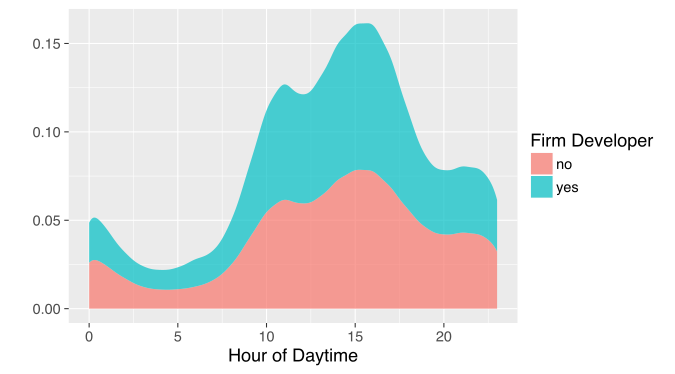
\includegraphics[page=1,scale=0.7]{../graphics/intro/hour_of_code_contribution_daytime_local.pdf}
	\caption{Code contributions of firm employed and external developers by local daytime (workdays, weekend and holidays are included). Most of the code commits are placed between 09:00 - 19:00, with its peak between 15:00 - 16:00}
	\label{fig:distribution_developer_commits_local}
\end{figure}

\begin{figure}[!ht]
	\centering
	\includegraphics[scale=0.4]{../graphics/images/us_standard_workday.png}
	\caption{2011-2012 Annual Averages ("Computer and Mathematical" (yellow) compared to "All Jobs" (green)): \textit{The majority of people are at work from 9:00 to 17:00, with a small break in the middle of the day for lunch} (according to \cite{TheAmericanWorkdayInOneGraph:online}). \footnotesize{Source: BLS, American Time Use Survey; Credit: Quoctrung Bui/NPR}}
	\label{fig:us_standard_workday}
\end{figure}

\clearpage
\subsection{Observed Repositories}

The final number of observed repositories is 3,419, including 610 top projects and 2,809 residual projects (see table \ref{tbl:overviewrepositories} for further details).

\begin{table}[!ht] \centering
	\footnotesize
	
% Table created by stargazer v.5.2 by Marek Hlavac, Harvard University. E-mail: hlavac at fas.harvard.edu
% Date and time: Sat, Mar 12, 2016 - 20:59:40

\begin{tabular}{@{\extracolsep{5pt}}lccccc}
\\[-1.8ex]\hline
\hline \\[-1.8ex]
Statistic & \multicolumn{1}{c}{N} & \multicolumn{1}{c}{Mean} & \multicolumn{1}{c}{St. Dev.} & \multicolumn{1}{c}{Min} & \multicolumn{1}{c}{Max} \\
\hline \\[-1.8ex]
Age (in days) & 3,419 & 743.790 & 560.458 & 0 & 2,904 \\
Number of Contributors & 3,419 & 17.181 & 40.053 & 2 & 468 \\
Number of Commits & 3,419 & 748.581 & 8,510.597 & 2 & 428,840 \\
Number of Commits by firm employed developers & 3,419 & 250.875 & 1,501.224 & 0 & 56,624 \\
All Issues count & 3,419 & 20.836 & 75.842 & 1 & 1,884 \\
Closed Issues count & 3,419 & 2.817 & 18.725 & 0 & 706 \\
Open Issues count & 3,419 & 18.019 & 74.182 & 0 & 1,884 \\
Stars & 3,419 & 426.290 & 1,538.234 & 0 & 35,214 \\
Subscribers & 3,419 & 75.221 & 123.100 & 1 & 2,617 \\
Forks & 3,419 & 99.204 & 378.507 & 0 & 10,772 \\
Ratio (share of firm employed developers) & 3,419 & 0.521 & 0.348 & 0.000 & 1.000 \\
Mean share of Top Repositories & 3,419 & 0.178 & 0.383 & 0 & 1 \\
\hline \\[-1.8ex]
\end{tabular}
% \end{table}

	\caption{Statistic of observed GitHub Projects}
  \label{tbl:overviewrepositories}
\end{table}

The number of repositories (i.e. observations) will vary between statistical models \footnote{some are using "Top Repositories", "Residual Repositories", "All Repositories" and "Repositories older than X days" for instance}.

\subsection{The Role of Developers on Issues}

\textit{Issues} are communication channels for GitHub repositories. GitHub provides data of users who opened issues and users who participate on issues by commenting / discussing. All comments will be counted and assigned to firm employed and external developers \footnote{some models also include a measurement of weighted comments by its content size}.

As mentioned before, issues can:

\begin{itemize}
	\item be technical (bug reports / source code related)
	\item include general ideas / feature requests
	\item be organizational related
\end{itemize}

Finally, we have 405,163 issues with 1,718,363 comments (6,190 issues and 32,599 issues' comments are by firm employed developers).

\subsection{Firms' OS Commitment as Proxy for Quality of Work Environment}

\label{sec:glassdoor_ratings}

To which extend does contribution of firm employees on firms' OS projects reflect the employer quality? If employed developers get encouraged by their employer to initiated and contribute on OS project, do they stay more likely at their current employer or rate their working climate more positive? If an firm employed developer is allowed to work on OS projects as part of his work, does it increase their incentive to be more creative and try out new ideas by themselves? Or do developers initiate projects to demonstrate and promote a specific technology innovation inside a firm?

This research question itself would probably fill another study (see \ref{sec:further_research}). But we will observe briefly a few data collections regarding to work climate and GitHub activities of firms. For that, ratings from employees of their workplace are evaluated. The data is received from Glassdoor. Ratings of 50 firms were found \footnote{\url{https://git.zeitpulse.com/philipp/masterthesis-data/tree/master/apidata/glassdoor/employers}} but only 14 firms (see table \ref{tbl:glassdoor_firm_ratings}) had enough ratings and enough Top Repositories (i.e. at least 38 ratings and 10 Top Repositories) to be "representative" with partly significant regression results. However, there is a (weak) positive significant relation between the number of popular OS projects and the rating by the employees (and vice versa) which could be measured by \textit{employees rating their firm} and \textit{firms' number of popular Open Source projects on GitHub} through the OLS method (see table \ref{tbl:glassdoorfirmratingandosprojects} for details). Interpretation: (a) if a firm initiates more OS projects, the firm is more valuable as employer for developers (b) if a firm is a good place to work, employees will more likely initiate OS projects through the firm.

Thus, the numbers of observations / ratings are not representative and might be a promising approach for further research.

\begin{table}[!h] \centering
	\scriptsize{
	
% Table created by stargazer v.5.2 by Marek Hlavac, Harvard University. E-mail: hlavac at fas.harvard.edu
% Date and time: Mi, Feb 10, 2016 - 20:05:53
\begin{tabular}{@{\extracolsep{5pt}}lcccc}
\\[-1.8ex]\hline
\hline \\[-1.8ex]
 & \multicolumn{4}{c}{\textit{Dependent variable:}} \\
\cline{2-5}
\\[-1.8ex] & Rating & OS Projects & Ratings count & Work-Life-Balance \\
\\[-1.8ex] & (1) & (2) & (3) & (4)\\
\hline \\[-1.8ex]
 Average Ratio Top Projects & $-$0.115 & 12.263 & 4,441.273 & 0.222 \\
  & (0.226) & (21.167) & (5,659.478) & (0.446) \\
  & & & & \\
 Average Ratio Residual Projects & 0.108 & $-$21.155 & $-$386.364 & $-$0.342 \\
  & (0.217) & (18.723) & (5,751.773) & (0.410) \\
  & & & & \\
 Ratings Count & 0.00003$^{*}$ & $-$0.002 &  & $-$0.00004 \\
  & (0.00001) & (0.001) &  & (0.00003) \\
  & & & & \\
 Rating &  & 74.312$^{**}$ & 17,654.490$^{*}$ & 1.638$^{**}$ \\
  &  & (25.873) & (8,434.416) & (0.486) \\
  & & & & \\
 Culture and Values & 0.634$^{***}$ & $-$37.375 & $-$13,061.970$^{*}$ & $-$0.769 \\
  & (0.132) & (24.268) & (5,587.065) & (0.510) \\
  & & & & \\
 Work-Life-Balance & 0.424$^{**}$ & $-$42.472$^{***}$ & $-$7,375.867 &  \\
  & (0.126) & (9.910) & (4,863.693) &  \\
  & & & & \\
 Age of Firm on GitHub & $-$0.0001 & 0.014$^{**}$ & 0.728 & 0.0003$^{**}$ \\
  & (0.0001) & (0.004) & (2.016) & (0.0001) \\
  & & & & \\
 OS Projects count & 0.008$^{**}$ &  & $-$142.543 & $-$0.019$^{***}$ \\
  & (0.003) &  & (104.811) & (0.004) \\
  & & & & \\
 Residual Repos. count & $-$0.001$^{**}$ & 0.152$^{***}$ & 26.620 & 0.003$^{***}$ \\
  & (0.0005) & (0.018) & (15.218) & (0.001) \\
  & & & & \\
 Constant & 0.024 & $-$4.067 & 7,961.749 & $-$0.065 \\
  & (0.338) & (31.831) & (7,988.258) & (0.665) \\
  & & & & \\
\hline \\[-1.8ex]
Observations & 14 & 14 & 14 & 14 \\
R$^{2}$ & 0.985 & 0.957 & 0.891 & 0.955 \\
Adjusted R$^{2}$ & 0.962 & 0.889 & 0.718 & 0.884 \\
Residual Std. Error (df = 5) & 0.076 & 7.202 & 1,975.574 & 0.150 \\
F Statistic (df = 8; 5) & 41.895$^{***}$ & 14.067$^{***}$ & 5.135$^{**}$ & 13.407$^{***}$ \\
\hline
\hline \\[-1.8ex]
\textit{Note:}  & \multicolumn{4}{r}{$^{*}$p$<$0.1; $^{**}$p$<$0.05; $^{***}$p$<$0.01} \\
\end{tabular}

	}
	\caption{Rating of Work Environment by employees and Firms' activity on Open Source projects}
  \label{tbl:glassdoorfirmratingandosprojects}
\end{table}

\clearpage

\subsection{Microsoft and GitHub Inc.: Contribution and Social Success Metrics of Atom and VSC}
\label{sec:atom_vs_vsc}

\begin{table}[!h]
\footnotesize{
\centering
\begin{tabular}{rllllllrllll}
  \hline
 & Init. by Firm & Editor & License & Stars & Subscr. & Forks & Contrib. & Published & Op.Issues & Commits & Ratio \\
  \hline
1 & GitHub & Atom & MIT & 23,998 & 1,524 & 4,094 & 260 & 2014 Q2 & 1,644 & 27,373 & 73.63\% \\
  2 & Microsoft & VSC & MIT & 9,884 & 679 & 1,205 &  56 & 2015 Q2 & 774 & 1,909 & 58.87\% \\
   \hline
\end{tabular}
\label{tbl:dataofvscodeandatom}
\caption[Repository Data of Atom and VSC]{Repository Data of Atom and VSC \protect\footnotemark}
}
\end{table}
\footnotetext{\ \ Retrieved on: \nth{21} January 2016 via \url{https://github.com/}}

The time series \ref{fig:codecontributionatomeditor} and \ref{fig:codecontributionvsc} \footnote{Retrieved on \nth{18} January 2016 via 'git log'} show the code contribution of \textit{GitHub} / \textit{Microsoft} employed developers against \textit{external developers}. \textbf{Gold} represents code contribution by external developers, \textbf{Black} represents code contribution by firm employed developers. \textit{Atom} was published as open source in May 2015, \textit{VSC} a half year later in November 2015.

If you compare the basic statistics of the competitors \textit{Microsoft} and \textit{GitHub Inc.} (see table \ref{tbl:summary_microsoft} and \ref{tbl:summary_github} on page \pageref{tbl:summary_microsoft}) you can see that \textit{Microsoft} is a "youngster" on \textit{GitHub} \footnote{the following values are mean values of each firms' projects}: Microsoft projects have a mean age of less than 1 year, high share of firm employed developers (over 68 \%) and fewer "Top Projects" (18 \% of Microsofts' projects are "Top Projects"). Whereas \textit{GitHub Inc.'s} "Top Project" share is 40 \% with a lower share of firm employed developers (53 \%) and older projects (mean age is almost 2 years).

\textbf{Interpretation:} This basic statistic provides indications of the differences between the two companies \textit{GitHub Inc.} and \textit{Microsoft}: Microsoft is a "newer" member of the OS community (according to the age of projects) and tries to gain its reputation (by initial high share of firm employed developers) and tries to establish popular projects (share of "Top Projects") with the long-range objective to motivate external developers (i.e. the OS community) to participate on their projects.

\begin{figure}[!h]
	\centering
	\includegraphics[page=1,scale=0.5]{../graphics/plots/timeseries/atom_vs_vscode/timeseries_repos_atom.pdf}
	\caption{Code Contribution of "Firm employed Developers" (int) and "External Developers" (ext) to Atom (GitHub Inc.). Published as open source in May 2015}
	\label{fig:codecontributionatomeditor}
\end{figure}

\begin{figure}[!h]
	\centering
	\includegraphics[page=1,scale=0.5]{../graphics/plots/timeseries/atom_vs_vscode/timeseries_repos_vscode.pdf}
	\caption{Code Contribution of "Firm employed Developers" (int) and "External Developers" to Visual Studio Code (Microsoft). Published as open source in November 2015. (time range of plot: Nov. 2015 - Jan. 2016)}
	\label{fig:codecontributionvsc}
\end{figure}
